\section{Programme}
\subsection{Systemcall \prgc{sys_execve}}
sucht und öffnet spezifizierte Datei\\
zählt und kopiert Argumente/Umgebungsvariablen\\
Request an jeden Binary Handler\\
Binary Handler versucht Datei zu laden \& interpretieren, wenn erfolgreich $\rightarrow$ Programm ausführen

\subsection{Executable and Linking Format (ELF)}
Binärformat, das Kompilate spezifiziert\\
Object-Files: \textcolor{green}{Linking View}, Programme: \textcolor{red}{Execution View}\\
Shared Objects (dynamische Bibliotheken): \textcolor{green}{Linking}/\textcolor{red}{Execution View}\\
Compiler erzeugt \textcolor{green}{Sektionen}, Linker \textcolor{red}{Segmente} (verschmilzt Sektionen gleicher Namens versch. Object-Files)\\
Loader sieht nur \textcolor{red}{Segmente}\\
\textbf{Header (52 Byte):} Typ, 32-bit/64-bit, endianess, maschine, entrypoint (zeigt, wo Programm gestartet werden muss), relative Adresse/Anzahl/Grösse Einträge der Tables
%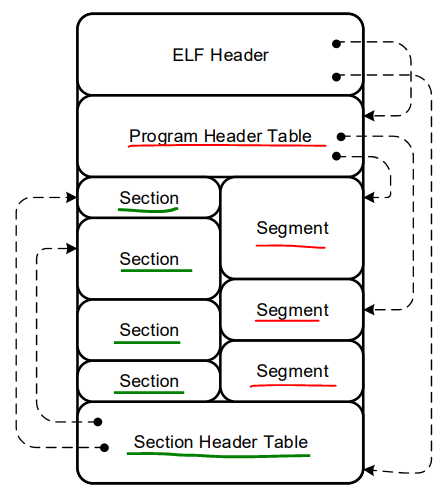
\includegraphics[scale = 0.3]{grafiken/ELF.PNG}\\
\textcolor{red}{\textbf{Program Header Table:}} Einträge zu 32 Byte; Einträge: Segment-Typ/Flags, Offset/Grösse der Datei, Virtuelle Adresse/Grösse im Speicher\\
\textcolor{green}{\textbf{Section Header Table:}} Einträge zu 40 Byte; Einträge: \underline{Name}(Referenz auf String Table), Typ/Flags, Offset/Grösse der Datei, Infos spezifisch für Typ\\
\textbf{String-Tabelle:} Namen von Symbolen, keine String-Literale aus Programm(in \prgc{.rodata})

